\documentclass[]{article}
\usepackage{lmodern}
\usepackage{amssymb,amsmath}
\usepackage{ifxetex,ifluatex}
\usepackage{fixltx2e} % provides \textsubscript
\ifnum 0\ifxetex 1\fi\ifluatex 1\fi=0 % if pdftex
  \usepackage[T1]{fontenc}
  \usepackage[utf8]{inputenc}
\else % if luatex or xelatex
  \ifxetex
    \usepackage{mathspec}
  \else
    \usepackage{fontspec}
  \fi
  \defaultfontfeatures{Ligatures=TeX,Scale=MatchLowercase}
\fi
% use upquote if available, for straight quotes in verbatim environments
\IfFileExists{upquote.sty}{\usepackage{upquote}}{}
% use microtype if available
\IfFileExists{microtype.sty}{%
\usepackage{microtype}
\UseMicrotypeSet[protrusion]{basicmath} % disable protrusion for tt fonts
}{}
\usepackage[margin=1in]{geometry}
\usepackage{hyperref}
\hypersetup{unicode=true,
            pdftitle={Important Distributions},
            pdfborder={0 0 0},
            breaklinks=true}
\urlstyle{same}  % don't use monospace font for urls
\usepackage{color}
\usepackage{fancyvrb}
\newcommand{\VerbBar}{|}
\newcommand{\VERB}{\Verb[commandchars=\\\{\}]}
\DefineVerbatimEnvironment{Highlighting}{Verbatim}{commandchars=\\\{\}}
% Add ',fontsize=\small' for more characters per line
\usepackage{framed}
\definecolor{shadecolor}{RGB}{248,248,248}
\newenvironment{Shaded}{\begin{snugshade}}{\end{snugshade}}
\newcommand{\KeywordTok}[1]{\textcolor[rgb]{0.13,0.29,0.53}{\textbf{#1}}}
\newcommand{\DataTypeTok}[1]{\textcolor[rgb]{0.13,0.29,0.53}{#1}}
\newcommand{\DecValTok}[1]{\textcolor[rgb]{0.00,0.00,0.81}{#1}}
\newcommand{\BaseNTok}[1]{\textcolor[rgb]{0.00,0.00,0.81}{#1}}
\newcommand{\FloatTok}[1]{\textcolor[rgb]{0.00,0.00,0.81}{#1}}
\newcommand{\ConstantTok}[1]{\textcolor[rgb]{0.00,0.00,0.00}{#1}}
\newcommand{\CharTok}[1]{\textcolor[rgb]{0.31,0.60,0.02}{#1}}
\newcommand{\SpecialCharTok}[1]{\textcolor[rgb]{0.00,0.00,0.00}{#1}}
\newcommand{\StringTok}[1]{\textcolor[rgb]{0.31,0.60,0.02}{#1}}
\newcommand{\VerbatimStringTok}[1]{\textcolor[rgb]{0.31,0.60,0.02}{#1}}
\newcommand{\SpecialStringTok}[1]{\textcolor[rgb]{0.31,0.60,0.02}{#1}}
\newcommand{\ImportTok}[1]{#1}
\newcommand{\CommentTok}[1]{\textcolor[rgb]{0.56,0.35,0.01}{\textit{#1}}}
\newcommand{\DocumentationTok}[1]{\textcolor[rgb]{0.56,0.35,0.01}{\textbf{\textit{#1}}}}
\newcommand{\AnnotationTok}[1]{\textcolor[rgb]{0.56,0.35,0.01}{\textbf{\textit{#1}}}}
\newcommand{\CommentVarTok}[1]{\textcolor[rgb]{0.56,0.35,0.01}{\textbf{\textit{#1}}}}
\newcommand{\OtherTok}[1]{\textcolor[rgb]{0.56,0.35,0.01}{#1}}
\newcommand{\FunctionTok}[1]{\textcolor[rgb]{0.00,0.00,0.00}{#1}}
\newcommand{\VariableTok}[1]{\textcolor[rgb]{0.00,0.00,0.00}{#1}}
\newcommand{\ControlFlowTok}[1]{\textcolor[rgb]{0.13,0.29,0.53}{\textbf{#1}}}
\newcommand{\OperatorTok}[1]{\textcolor[rgb]{0.81,0.36,0.00}{\textbf{#1}}}
\newcommand{\BuiltInTok}[1]{#1}
\newcommand{\ExtensionTok}[1]{#1}
\newcommand{\PreprocessorTok}[1]{\textcolor[rgb]{0.56,0.35,0.01}{\textit{#1}}}
\newcommand{\AttributeTok}[1]{\textcolor[rgb]{0.77,0.63,0.00}{#1}}
\newcommand{\RegionMarkerTok}[1]{#1}
\newcommand{\InformationTok}[1]{\textcolor[rgb]{0.56,0.35,0.01}{\textbf{\textit{#1}}}}
\newcommand{\WarningTok}[1]{\textcolor[rgb]{0.56,0.35,0.01}{\textbf{\textit{#1}}}}
\newcommand{\AlertTok}[1]{\textcolor[rgb]{0.94,0.16,0.16}{#1}}
\newcommand{\ErrorTok}[1]{\textcolor[rgb]{0.64,0.00,0.00}{\textbf{#1}}}
\newcommand{\NormalTok}[1]{#1}
\usepackage{graphicx,grffile}
\makeatletter
\def\maxwidth{\ifdim\Gin@nat@width>\linewidth\linewidth\else\Gin@nat@width\fi}
\def\maxheight{\ifdim\Gin@nat@height>\textheight\textheight\else\Gin@nat@height\fi}
\makeatother
% Scale images if necessary, so that they will not overflow the page
% margins by default, and it is still possible to overwrite the defaults
% using explicit options in \includegraphics[width, height, ...]{}
\setkeys{Gin}{width=\maxwidth,height=\maxheight,keepaspectratio}
\IfFileExists{parskip.sty}{%
\usepackage{parskip}
}{% else
\setlength{\parindent}{0pt}
\setlength{\parskip}{6pt plus 2pt minus 1pt}
}
\setlength{\emergencystretch}{3em}  % prevent overfull lines
\providecommand{\tightlist}{%
  \setlength{\itemsep}{0pt}\setlength{\parskip}{0pt}}
\setcounter{secnumdepth}{0}
% Redefines (sub)paragraphs to behave more like sections
\ifx\paragraph\undefined\else
\let\oldparagraph\paragraph
\renewcommand{\paragraph}[1]{\oldparagraph{#1}\mbox{}}
\fi
\ifx\subparagraph\undefined\else
\let\oldsubparagraph\subparagraph
\renewcommand{\subparagraph}[1]{\oldsubparagraph{#1}\mbox{}}
\fi

%%% Use protect on footnotes to avoid problems with footnotes in titles
\let\rmarkdownfootnote\footnote%
\def\footnote{\protect\rmarkdownfootnote}

%%% Change title format to be more compact
\usepackage{titling}

% Create subtitle command for use in maketitle
\newcommand{\subtitle}[1]{
  \posttitle{
    \begin{center}\large#1\end{center}
    }
}

\setlength{\droptitle}{-2em}

  \title{Important Distributions}
    \pretitle{\vspace{\droptitle}\centering\huge}
  \posttitle{\par}
    \author{}
    \preauthor{}\postauthor{}
    \date{}
    \predate{}\postdate{}
  

\begin{document}
\maketitle

\subsection{Discrete Distribution}\label{discrete-distribution}

\subsubsection{Bonomial Distribution}\label{bonomial-distribution}

``The binomial distribution fits to repeated trials each with a
dichotomous out-come such as succes-failure, healthy-disease,
heads-tails, purine-pyrimidine, etc. When there are n trials, then the
number of ways to obtain k successes out of n is given by the binomial
coefficient''

\begin{verbatim}
                                    n!/k!(n-k)!
\end{verbatim}

\begin{Shaded}
\begin{Highlighting}[]
\CommentTok{# uncomment to see the binomial distribution}
\CommentTok{#TeachingDemos::vis.binom()}
\end{Highlighting}
\end{Shaded}

To use the formula to find the probability of an event:

\begin{figure}
\centering
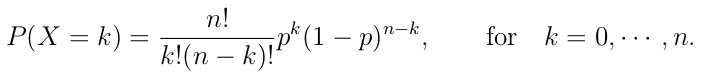
\includegraphics{binomial.png}
\caption{}
\end{figure}

\paragraph{Example: Albinism}\label{example-albinism}

\begin{verbatim}
If two carriers of the gen for albinism marry, then each of the children has probability of 1/4 of being albino. What is the probability for one child out of three to be albino?
\end{verbatim}

R has a function to calculate the probabilty of a binomial: dbinom

\begin{Shaded}
\begin{Highlighting}[]
\CommentTok{# we know that...}
\NormalTok{p =}\StringTok{ }\FloatTok{0.25}

\CommentTok{# we know they'll have 3 kids}
\NormalTok{n =}\StringTok{ }\DecValTok{3}

\CommentTok{# we're asked the odds for k = 1 }
\NormalTok{k =}\StringTok{ }\DecValTok{1}

\CommentTok{# just pass it to dbinom:}
\KeywordTok{dbinom}\NormalTok{(k, n, p)}
\end{Highlighting}
\end{Shaded}

\begin{verbatim}
## [1] 0.421875
\end{verbatim}

This gives use about 42\%.

\begin{verbatim}
  What are the odds that all 2 or fewer are albino?
\end{verbatim}

This is calculated by summing the probabilities of the ks up to the one
in question, ie:

\begin{Shaded}
\begin{Highlighting}[]
\CommentTok{# up the results form 0 to n}
\KeywordTok{dbinom}\NormalTok{(}\DecValTok{0}\NormalTok{, n, p) }\OperatorTok{+}\StringTok{ }\KeywordTok{dbinom}\NormalTok{(}\DecValTok{1}\NormalTok{, n, p) }\OperatorTok{+}\StringTok{ }\KeywordTok{dbinom}\NormalTok{(}\DecValTok{2}\NormalTok{, n, p)}
\end{Highlighting}
\end{Shaded}

\begin{verbatim}
## [1] 0.984375
\end{verbatim}

You can do this with a for-loop or use the pbinom function:

\begin{Shaded}
\begin{Highlighting}[]
\CommentTok{# odds ot two or fewer }
\KeywordTok{pbinom}\NormalTok{(}\DecValTok{2}\NormalTok{, n, p)}
\end{Highlighting}
\end{Shaded}

\begin{verbatim}
## [1] 0.984375
\end{verbatim}

This relationship can be visualized like this:

\begin{figure}
\centering
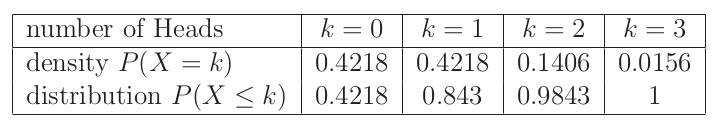
\includegraphics{probTable.png}
\caption{}
\end{figure}

\paragraph{Example: RNA Micro-array}\label{example-rna-micro-array}

\begin{verbatim}
RNA consists of a sequence of nucleotides A, G, U, and C, where the first two are purines and the last two are pyrimidines. Suppose, for the purpose of illustration, that the length of a certain micro RNA is 22, that the probability of a purine equals 0.7, and that the process of placing purines and pyrimidines is binomially distributed. The event that our microRNA contains 14 purines can be represented by X = 14. The probability of this event can be computed by

  n = 22
  Puries: A,G (p = 0.7)
  Pyrimidines: U,C (p = 0.3)
  
\end{verbatim}

\begin{Shaded}
\begin{Highlighting}[]
\CommentTok{# the long way}
\NormalTok{(}\KeywordTok{factorial}\NormalTok{(}\DecValTok{22}\NormalTok{)}\OperatorTok{/}\NormalTok{(}\KeywordTok{factorial}\NormalTok{(}\DecValTok{14}\NormalTok{)}\OperatorTok{*}\StringTok{ }\KeywordTok{factorial}\NormalTok{(}\DecValTok{22}\OperatorTok{-}\DecValTok{14}\NormalTok{))) }\OperatorTok{*}\StringTok{ }\NormalTok{(}\FloatTok{0.7}\OperatorTok{^}\DecValTok{14}\NormalTok{)}\OperatorTok{*}\NormalTok{(}\FloatTok{0.3}\OperatorTok{^}\NormalTok{(}\DecValTok{22}\OperatorTok{-}\DecValTok{14}\NormalTok{))}
\end{Highlighting}
\end{Shaded}

\begin{verbatim}
## [1] 0.1422919
\end{verbatim}

\begin{verbatim}
What about the odds there are 13 or fewer?
\end{verbatim}

\begin{Shaded}
\begin{Highlighting}[]
\CommentTok{# use the function as before}
\KeywordTok{pbinom}\NormalTok{(}\DecValTok{13}\NormalTok{, }\DecValTok{22}\NormalTok{, }\FloatTok{0.7}\NormalTok{)}
\end{Highlighting}
\end{Shaded}

\begin{verbatim}
## [1] 0.1864574
\end{verbatim}

\begin{verbatim}
The odds of ten or more?
\end{verbatim}

\begin{Shaded}
\begin{Highlighting}[]
\CommentTok{# use dbinom}
\KeywordTok{sum}\NormalTok{(}\KeywordTok{dbinom}\NormalTok{(}\DecValTok{11}\OperatorTok{:}\DecValTok{22}\NormalTok{, }\DecValTok{22}\NormalTok{, }\FloatTok{0.7}\NormalTok{))}
\end{Highlighting}
\end{Shaded}

\begin{verbatim}
## [1] 0.9859649
\end{verbatim}

\paragraph{Visualizing the
Distributions}\label{visualizing-the-distributions}

\begin{Shaded}
\begin{Highlighting}[]
\NormalTok{desiredRange <-}\StringTok{ }\DecValTok{1}\OperatorTok{:}\DecValTok{22}

\KeywordTok{plot}\NormalTok{(desiredRange, }\KeywordTok{dbinom}\NormalTok{(desiredRange, }\DataTypeTok{size =} \DecValTok{22}\NormalTok{, }\DataTypeTok{prob =} \FloatTok{0.7}\NormalTok{), }\DataTypeTok{type =} \StringTok{"h"}\NormalTok{)}
\end{Highlighting}
\end{Shaded}

\includegraphics{ch3_content_files/figure-latex/Visualiz Distributions-1.pdf}

\subsection{Continuous Distribution}\label{continuous-distribution}

\subsubsection{Chi-Square}\label{chi-square}

The Chi-Square distribution is used to test hypothesis about
feequencies. It is defined as the sum of a set of the squared value of a
set of random independent variables, with \emph{m} degrees of freedom:

\begin{figure}
\centering
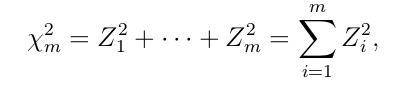
\includegraphics{chiSquared.PNG}
\caption{}
\end{figure}


\end{document}
